
\documentclass[fleqn,usenatbib]{mnras}

\usepackage{newtxtext,newtxmath}
\usepackage[T1]{fontenc}

\DeclareRobustCommand{\VAN}[3]{#2}
\let\VANthebibliography\thebibliography
\def\thebibliography{\DeclareRobustCommand{\VAN}[3]{##3}\VANthebibliography}


%%%%% AUTHORS - PLACE YOUR OWN PACKAGES HERE %%%%%


\usepackage{graphicx}
\usepackage{amsmath}

\title{Tidal Evolution of M33’s Dark Matter Halo}

\author{
Aidan DeBrae$^{1}$
\\
% List of institutions
$^{1}$Department of Astronomy, University of Arizona, 933 North Cherry Avenue, Tucson, AZ, 85719}

% Don't change these lines
\begin{document}
\label{firstpage}
\pagerange{\pageref{firstpage}--\pageref{lastpage}}
\maketitle

% Select between one and six entries from the list of approved keywords.
% Don't make up new ones.
\begin{keywords}
Local Group -- Dark Matter Halo -- Galaxy Merger -- Cold Dark Matter Theory -- Satellite Galaxy -- Halo Shape -- Hernquist Profile
\end{keywords}

%%%%%%%%%%%%%%%%%%%%%%%%%%%%%%%%%%%%%%%%%%%%%%%%%%

%%%%%%%%%%%%%%%%% BODY OF PAPER %%%%%%%%%%%%%%%%%%

\section{Introduction}
\hspace{6mm}Observations of our cosmic structure continually present evidence which further support the theoretical model that indicates our universe is primarily composed of Dark Matter (DM). Although there are many theories about what dark matter could actually be it is generally concluded it is a source of matter which has little to no interaction with baryonic matter except through gravity. Almost all of the evidence which supports the the presence of DM comes from observing the structure and behavior of galaxies. A particularly strong piece of observational evidence for dark matter is the affect of gravitational lensing. Due to their immense gravitational potential galaxies are capable of distorting light such that we can use the curvature of the light to calculate the mass of the galaxy. \citep{Massey_2010}. The results consistently show that galaxies contain significantly more mass than just the observed baryonic matter. This is further supported by physical characteristics of the galaxy like the rotation curve. Measurements of rotation curves indicate the presence of dark matter because rather than a bell shaped distribution in which the rotational velocity displays a peak and then falls off toward the edge of the galaxy the curve exhibits a nearly flat velocity distribution throughout the majority of the galaxy \citep{Hoeneisen19}. This indicates there is a very large source of mass which extends beyond the edges of the halo. It is important to consider the potential consequences of the influence of dark matter halos. The evidence clearly proves the effects of dark matter halos can dramatically impact the physical characteristics of a galaxy. It would thus be reasonable to conclude DM might influence other properties of the galaxy like orbital kinematics, star formation, and even the super massive black hole at the center of the galaxy \citep{Springel05}. If the dark matter halo is expected to play such an important role in galactic evolution it is critical to investigate the the structure and behavior of the halo. Conveniently, observations have allowed astrophysicists to determine the fate of the Local Group system which might provide some understanding of how dark matter behaves. In roughly 4 billion years the Local Group will experience a catastrophic event. That event is when our own galaxy, the Milky Way (MW), will collide with our closest neighboring galaxy, Andromeda (M31). The collision of these two galaxies will produce immense changes to their own structure as well as any nearby satellite galaxies. It follows that the dark matter halos which surround these galaxies will also undergo immense changes. Using simulations, an analysis of the shape and density profile of the halos as this collision event occurs will offer insight into how the structure of the halo changes over time. 

 \hspace{6mm}To investigate the relationship between galaxies and their dark matter halos it is best to first carefully define the broad terms associated with them. A galaxy is defined by \cite{Willman12} as ``[...] a gravitationally bound set of stars whose properties cannot be explained by a combination of baryons (gas \& stars) and Newton's laws of gravity.'' Due to the complexity of galaxy evolution it is quite difficult to precisely define what it means. An excellent general description is provided by \cite{Mo10} where galaxy evolution is defined by "[...] comparing [galaxy] properties, in a statistical sense, at different epochs." This definition motivates the exploration of the Local Group dark matter halos since it has been firmly established by observations that dark matter plays an important role in determining the properties of the galaxy it surrounds. Additionally, the collision of the MW \& M31 in the future provides a tightly constrained system in which the properties of the galaxies and their halos can be constructed in N-body simulations to predict how both the individual galaxies and the Local Group will evolve over time. Simulations have shown that the properties of dark matter effect the morphology of galaxies over time \citep{Cataldi21}. This is further accentuated by \cite{Chua22} as their research concluded there is a strong relationship between the properties of the halo shape and baryonic matter stating, ``[...] the change in halo shape depends on aspects of the baryonic physics; e.g. gas cooling, star formation and galactic feedback. By considering a variety of galactic feedback models, we showed that the correlation between halo shape and stellar mass fraction is consistent even when baryonic physics are modified in the simulations.'' Thus, understanding the shape of a halo is vital in developing a clear picture of the relationship between a galaxy and its surrounding dark matter. As stated previously, research suggests this relationship might play an important role in how a galaxy evolves over time.    

\hspace{6mm}Research regarding the shape of dark matter halos has been primarily directed at the MW and its satellite galaxies. Very little is known about the structure of M31 and its nearby satellites. The reason efforts have been focused on the MW system is because the Large Magellenic Cloud (LMC) has recently collided with the MW galaxy \citep{Choi_2022}. Because this event happened so recently, the baryonic matter of the galaxy interaction still displays the physical features that would result from a galactic collision. This is incredibly valuable when investigating the galaxy-halo relationship as it allows simulations to compare results with the observational data of the real system. Normally, astronomical time scales make it nearly impossible to directly observe radical cosmic events like two galaxies colliding. Taking advantage of this rare occurrence astrophysicists have been particularly interested in modelling the dark matter halo system in hopes of developing a more clear understanding of how the structure of the halos might effect the galaxies. According to \cite{Garavito-Camargo_2021} N-body simulations have shown that, ``[..] the DM halo shape/distribution contains information about the location and amplitude of the DM dynamical friction wake.'' The debris of DM generated by the collision of the MW and the LMC will result in a wake caused by dynamical friction. This likely will have the most significant gravitational influence over the baryonic matter and could help relate the behavior of the halo to the galaxy. Based on the claims made by \cite{Garavito-Camargo_2021} it would be incredibly useful to be able to characterize the shape of the halo. If the shape of the halo can be used to determine the location of a dynamical friction wake it could shed light on previous interactions in different systems and help construct a more detailed comprehension of galactic evolution. In an attempt to accurately characterize the halo shapes \cite{Garavito-Camargo_2021} used the gravitational energy of the halos to compare them to idealized prolate, oblate, and triaxial halo shapes. These will be more precisely defined in section \ref{Method}. Unfortunately, simulations have not yet been successful in concluding whether or not our models of the dark matter halos reflect any of the ideal shapes. As of now, the simulations show halos which are much too chaotic to accurately constrain. Although much more is being learned about the importance of halo shape there is still a lot of work to be done to understand the details of the halo-galaxy relationship. \cite{Chua22} comes to the conclusion that ``[...] a larger observational sample would be required to statistically distinguish between different baryonic prescriptions due to large halo-to-halo variation in halo shapes.'' More observations of galaxies directed at understanding the potential relationship between baryonic and dark matter could help theorists develop more accurate models for determining the shapes of halos and their effects.

\hspace{6mm} HAVING TROUBLE WITH PARAGRAPH 4. Admittedly, I am at a bit of road block with this paragraph. I don't really feel like know exactly what the open questions are without being simple and saying something about the fact we don't really know the shape of dark matter halos. I think I have gotten a lot of good resources about this topic but I'm having a hard time formulating this overarching discussion of halo shape and structure and what sort of big picture questions might be related to the topic. I think part of the issue with this paragraph is feeling like the things I would say would be redundant to what I have already discussed above. Should I make the above paragraphs shorter and work in some of the concepts here? Or did I construct some decent paragraphs above and potentially just need some help formulating the right questions? I would love some direction here. IDEAS: How does a more massive system like the Mw M31 collision effect the shape of satellite halos? How do the tidal effects from their collision change the shape of the halo? Does a larger system provide more conclusive results for the halo shape? 


\section{Shape of the M33 Dark Matter Halo}
\hspace{6mm}This research paper focuses on the evolution of the dark matter halo of M31's most massive satellite galaxy, Triangulum (M33). More specifically, the research will investigate the tidal effects from the collision of MW \& M31 and how it contributes to the structural evolution of M33's dark matter halo. The primary structural feature which this report will explore in depth is the shape of the halo. Simulations of the MW-LMC system show that prolate, oblate, and triaxial shapes have different effects on the structure of the halo and in turn the baryonic matter of the galaxy.  

\hspace{6mm}A FEW NOTES. I'M LEAVING THE MAIN QUESTION FROM THE RESEARCH TOPIC PROMPT AS A MEANS OF KEEPING TRACK OF THE FOUNDATION OF THE REPORT. I INTEND ON TAKING THIS OUT AFTER I DEVELOP SOME BETTER WRITING ABOUT THE QUESTIONS. AS STATED PREVIOUSLY I'M AT A BIT OF A ROADBLOCK WITH PARAGRAPH 4 BUT I THINK I HAVE SOME SOLID IDEAS AS TO WHAT THE IMPORTANT MAIN QUESTIONS ARE FOR MY REPORT. First, I'd like to address the question "What is the shape of the dark matter distribution of M33? How does this change with time? Is it elongated/ellipsoid or spherical? What do terms like prolate, oblate, or triaxial halos mean?" I  believe the important questions surrounding the shape of the dark matter halo are as follows. How do the tidal effects from the MW M31 collision influence the shape of the M33 halo? What sort of influence does the shape of the halo have on the system? How does the a larger system like the collision between the MW \& M31 compare to smaller systems that have been investigated like the MW and its satellite galaxy the LMC? Does a larger system give more accurate results for the shape of the halo?

\hspace{6mm}It has already been established that the shape of dark matter halos can influence many aspects of a galaxy. However, most research into how the shape of dark matter halos influence galactic evolution has focused on halos and their satellite galaxy. In this case we are interested in the collision and eventual merger of the MW and M31 which is a much much larger system. If smaller dark matter halo systems are shown to impact the nature of their host halo it can be extrapolated that a very large system undergoing a catastrophic event could have even more dramatic impacts.


\section{Methodology} \label{Method}
I think the best approach to answering the first question involving the shape of the dark matter halo is reflected in lab 7. This lab demonstrates how a histogram and contour fitting can illustrate the shape of a astronomical object. This will be accomplished by extracting particle position data from the simulation. Of course, to analyze the evolution of the halo, I'll create many plots each according to the red-shift values as MW \& M31 approach each other and collide. Various pieces of code which we have developed over the course of the semester will prove useful such as the code which calculates the center of mass of a given halo. I NEED TO REWORK THE EXACT WRITING IN THIS SECTION BUT I FOUND THE EXACT CONSTRAINTS I WANT TO USE TO DEFINE THE SHAPE OF THE HALO. From \cite{Garavito-Camargo_2021} the ellipsoid axis ratios can be defined as $s_\rho = c/a$ for the minor to major axis ratio, and $q_\rho = b/a$ for the intermediate to major axis ratio. Using these definitions the triaxality of the halo can be defined as $T_{qs} = \frac{1-q_{\rho}^2}{1-s_{\rho}^2}$ where if $T_{qs} \ge 0.67$ is prolate, $0.67 \ge T_{qs} \ge 0.33$ is triaxial, and $T_{qs} \le 0.33$ is oblate. These are also shown by \ref{fig:shapes}


\begin{figure}
	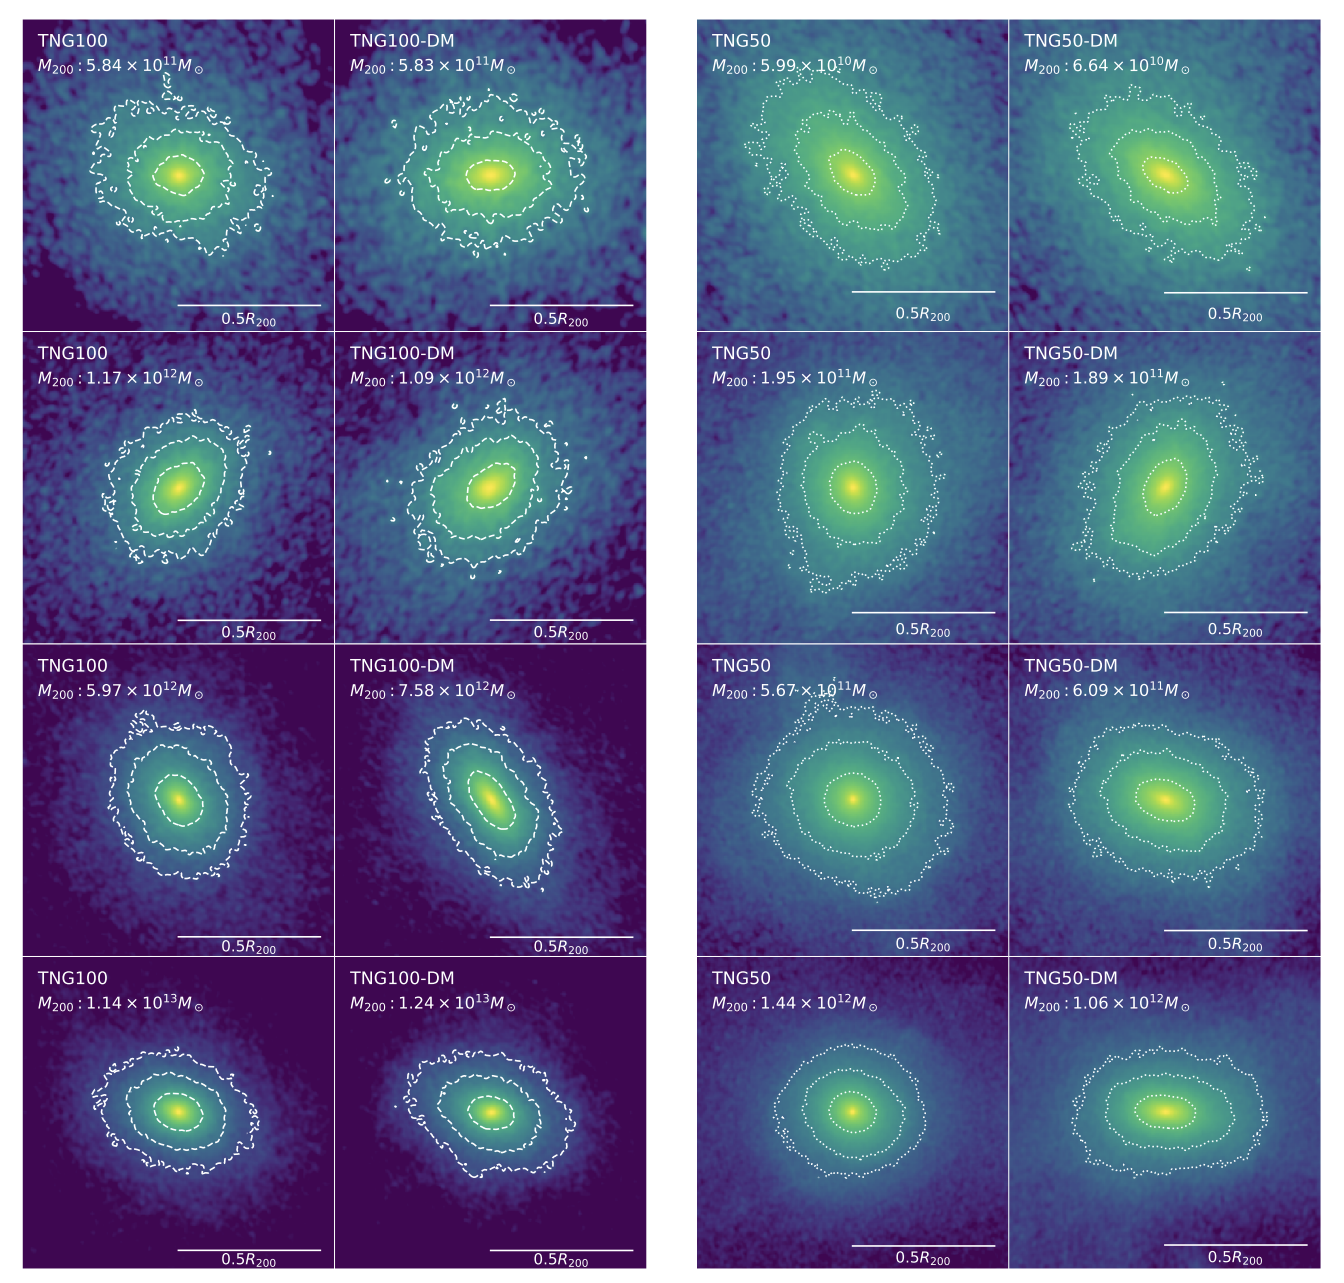
\includegraphics[width=\columnwidth]{density_countours.png}
    \caption{Example of the piece of code which creates a 2D density contour diagram}
    \label{fig:density_code}
\end{figure}
\begin{figure}
	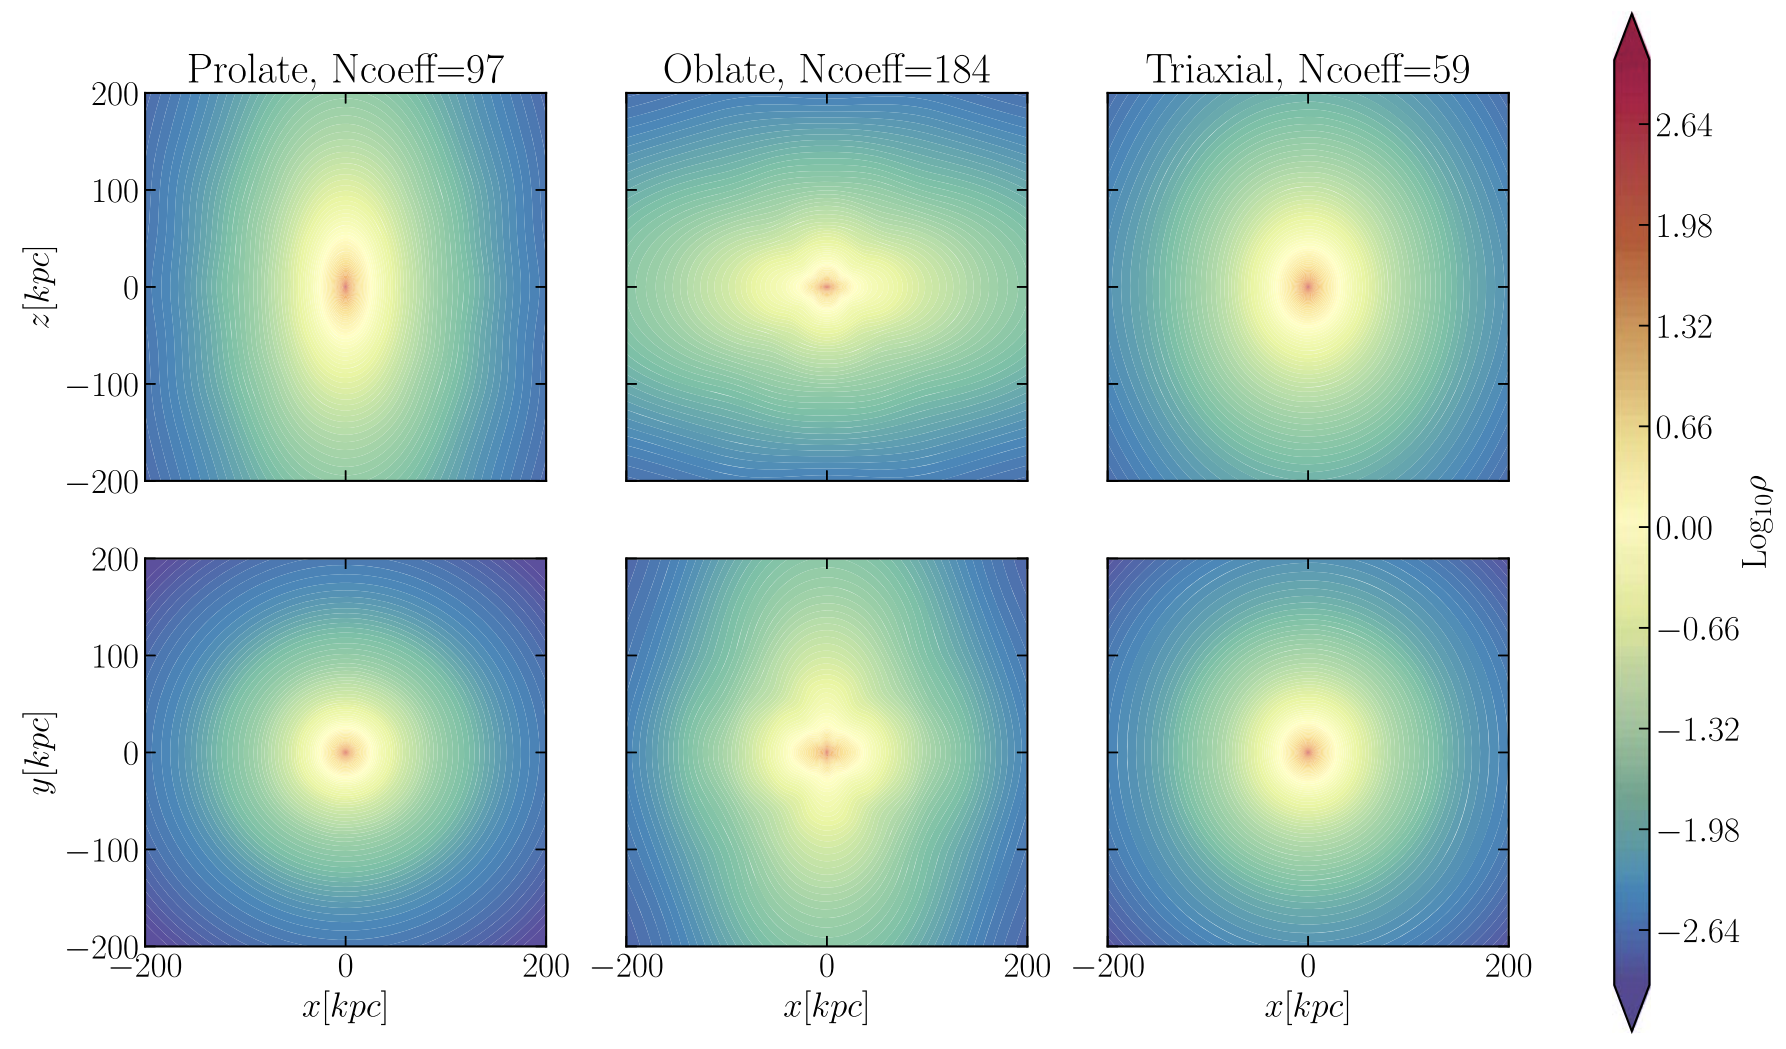
\includegraphics[width=\columnwidth]{2D_halo_shape.png}
    \caption{Ideal shapes and contour lines of the ideal shapes of the 2D projection.}
    \label{fig:shapes}
\end{figure}

I am going to plot the 2D projections of the halos to investigate the shapes. To best capture the shape of the halos I'll plot the halo during the pericenter and apocenter approach of M33 and M31. 
I SPENT A LOT OF TIME REVISING MY RESOURCES AND MAIN INTRODUCTION IN AN ATTEMPT TO CLEAN UP AND REDIRECT MY PAPER THAT SHOULD BETTER REFLECT MY TOPIC OF INTEREST. I ALSO WORKED ON UNDERSTANDING THE TOPIC AND THE PREVIOUS WORK RELATED TO IT. I THINK THIS MADE THE METHODOLOGY SUFFER A LITTLE BIT IT TERMS OF REVISIONS AND UPDATES. THE CODE I CREATED FOR THE LAST ASSIGNMENT HAS GIVEN ME A GOOD FEEL AS TO WHAT METHDOS ILL USE TO CALCULATE WHETHER OR NOT THE PHYSICAL FEATURES MATCH THE CONDITIONS IM GOING TO USE FROM THE PAPERS. I WILL CONTINUE WORKING ON THIS AND WOULD LIKE TO ATTEND SOME OFFICE HOURS TO IMPROVE THE PAPER. 

\subsection{Hypothesis}
I believe that M33's dark matter halo will start with a semi-spheroidal shape with a Hernquist density profile. As the halo evolves, I think it will begin to exhibit an oblate shape as the gravitational pull from tidal disruption caused by it's host halo and MW approaching one another. This will inevitably cause the density profile to change in which the density will become more concentrated toward the combined MW \& M31 dark matter halo. I believe the immense gravitational contribution from MW \& M31 will change the shape an density profile of M33. If it does not change that could mean that M33 is outside of the range of the tidal affects of their collision.   

\bibliographystyle{mnras}
\bibliography{RA_2_references} 



% Don't change these lines
\bsp	% typesetting comment
\label{lastpage}
\end{document}

% End of mnras_template.tex
